

\tikzset{every picture/.style={line width=0.75pt}} %set default line width to 0.75pt        

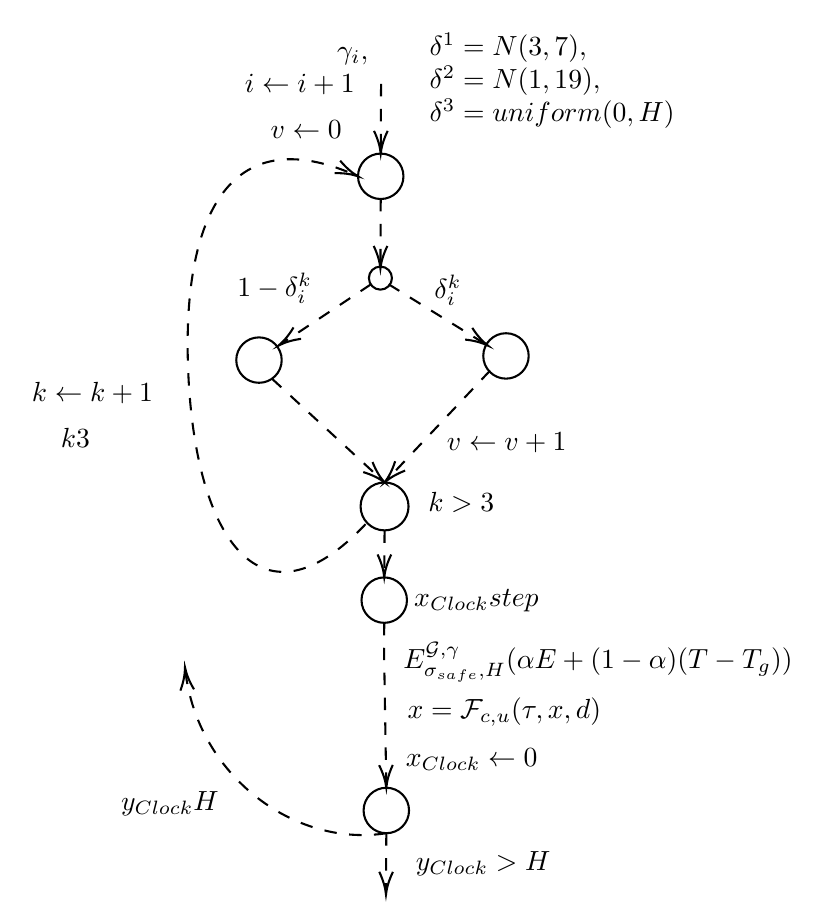
\begin{tikzpicture}[x=0.75pt,y=0.75pt,yscale=-1,xscale=1]
%uncomment if require: \path (0,460); %set diagram left start at 0, and has height of 460

%Shape: Circle [id:dp7284696639089192] 
\draw   (221.89,122.55) .. controls (221.89,119.49) and (224.38,117) .. (227.45,117) .. controls (230.51,117) and (233,119.49) .. (233,122.55) .. controls (233,125.62) and (230.51,128.11) .. (227.45,128.11) .. controls (224.38,128.11) and (221.89,125.62) .. (221.89,122.55) -- cycle ;
%Shape: Circle [id:dp7092344590230357] 
\draw   (217.89,232.55) .. controls (217.89,226.17) and (223.06,221) .. (229.45,221) .. controls (235.83,221) and (241,226.17) .. (241,232.55) .. controls (241,238.94) and (235.83,244.11) .. (229.45,244.11) .. controls (223.06,244.11) and (217.89,238.94) .. (217.89,232.55) -- cycle ;
%Straight Lines [id:da95053023471753] 
\draw  [dash pattern={on 4.5pt off 4.5pt}]  (229.45,244.11) -- (229.3,264.65) ;
\draw [shift={(229.29,266.65)}, rotate = 270.4] [color={rgb, 255:red, 0; green, 0; blue, 0 }  ][line width=0.75]    (10.93,-3.29) .. controls (6.95,-1.4) and (3.31,-0.3) .. (0,0) .. controls (3.31,0.3) and (6.95,1.4) .. (10.93,3.29)   ;
%Straight Lines [id:da6246395919086472] 
\draw  [dash pattern={on 4.5pt off 4.5pt}]  (227.6,84.45) -- (227.53,99.1) -- (227.46,116) ;
\draw [shift={(227.45,118)}, rotate = 270.27] [color={rgb, 255:red, 0; green, 0; blue, 0 }  ][line width=0.75]    (10.93,-3.29) .. controls (6.95,-1.4) and (3.31,-0.3) .. (0,0) .. controls (3.31,0.3) and (6.95,1.4) .. (10.93,3.29)   ;
%Shape: Circle [id:dp603073223077478] 
\draw   (158,162.05) .. controls (158,156.01) and (162.9,151.11) .. (168.95,151.11) .. controls (174.99,151.11) and (179.89,156.01) .. (179.89,162.05) .. controls (179.89,168.1) and (174.99,173) .. (168.95,173) .. controls (162.9,173) and (158,168.1) .. (158,162.05) -- cycle ;
%Shape: Circle [id:dp929274482174262] 
\draw   (277,160.05) .. controls (277,154.01) and (281.9,149.11) .. (287.95,149.11) .. controls (293.99,149.11) and (298.89,154.01) .. (298.89,160.05) .. controls (298.89,166.1) and (293.99,171) .. (287.95,171) .. controls (281.9,171) and (277,166.1) .. (277,160.05) -- cycle ;
%Straight Lines [id:da35420719147701685] 
\draw  [dash pattern={on 4.5pt off 4.5pt}]  (280.29,167.11) -- (257.95,190.79) -- (230.82,219.55) ;
\draw [shift={(229.45,221)}, rotate = 313.33000000000004] [color={rgb, 255:red, 0; green, 0; blue, 0 }  ][line width=0.75]    (10.93,-3.29) .. controls (6.95,-1.4) and (3.31,-0.3) .. (0,0) .. controls (3.31,0.3) and (6.95,1.4) .. (10.93,3.29)   ;
%Straight Lines [id:da4723956433829293] 
\draw  [dash pattern={on 4.5pt off 4.5pt}]  (175.29,171.11) -- (227.98,219.64) ;
\draw [shift={(229.45,221)}, rotate = 222.65] [color={rgb, 255:red, 0; green, 0; blue, 0 }  ][line width=0.75]    (10.93,-3.29) .. controls (6.95,-1.4) and (3.31,-0.3) .. (0,0) .. controls (3.31,0.3) and (6.95,1.4) .. (10.93,3.29)   ;
%Straight Lines [id:da5493223449601987] 
\draw  [dash pattern={on 4.5pt off 4.5pt}]  (231.45,125.55) -- (256.38,140.96) -- (277.59,154.06) ;
\draw [shift={(279.29,155.11)}, rotate = 211.7] [color={rgb, 255:red, 0; green, 0; blue, 0 }  ][line width=0.75]    (10.93,-3.29) .. controls (6.95,-1.4) and (3.31,-0.3) .. (0,0) .. controls (3.31,0.3) and (6.95,1.4) .. (10.93,3.29)   ;
%Straight Lines [id:da4708123952991736] 
\draw  [dash pattern={on 4.5pt off 4.5pt}]  (222.89,125.55) -- (179.96,154) ;
\draw [shift={(178.29,155.11)}, rotate = 326.47] [color={rgb, 255:red, 0; green, 0; blue, 0 }  ][line width=0.75]    (10.93,-3.29) .. controls (6.95,-1.4) and (3.31,-0.3) .. (0,0) .. controls (3.31,0.3) and (6.95,1.4) .. (10.93,3.29)   ;
%Shape: Circle [id:dp6748222746281551] 
\draw   (216.66,73.51) .. controls (216.66,67.46) and (221.56,62.56) .. (227.6,62.56) .. controls (233.65,62.56) and (238.55,67.46) .. (238.55,73.51) .. controls (238.55,79.55) and (233.65,84.45) .. (227.6,84.45) .. controls (221.56,84.45) and (216.66,79.55) .. (216.66,73.51) -- cycle ;
%Curve Lines [id:da3847758460174753] 
\draw  [dash pattern={on 4.5pt off 4.5pt}]  (220.29,241.11) .. controls (169.86,294.5) and (139.01,248.14) .. (135.01,171.02) .. controls (131.02,94.28) and (153.56,45.44) .. (215.72,73.09) ;
\draw [shift={(216.66,73.51)}, rotate = 204.43] [color={rgb, 255:red, 0; green, 0; blue, 0 }  ][line width=0.75]    (10.93,-3.29) .. controls (6.95,-1.4) and (3.31,-0.3) .. (0,0) .. controls (3.31,0.3) and (6.95,1.4) .. (10.93,3.29)   ;
%Straight Lines [id:da47628861649753884] 
\draw  [dash pattern={on 4.5pt off 4.5pt}]  (227.76,29.02) -- (227.69,43.66) -- (227.61,60.56) ;
\draw [shift={(227.6,62.56)}, rotate = 270.27] [color={rgb, 255:red, 0; green, 0; blue, 0 }  ][line width=0.75]    (10.93,-3.29) .. controls (6.95,-1.4) and (3.31,-0.3) .. (0,0) .. controls (3.31,0.3) and (6.95,1.4) .. (10.93,3.29)   ;
%Shape: Circle [id:dp48342387303657786] 
\draw   (218.34,277.71) .. controls (218.34,271.66) and (223.24,266.76) .. (229.29,266.76) .. controls (235.34,266.76) and (240.24,271.66) .. (240.24,277.71) .. controls (240.24,283.75) and (235.34,288.65) .. (229.29,288.65) .. controls (223.24,288.65) and (218.34,283.75) .. (218.34,277.71) -- cycle ;
%Straight Lines [id:da7144351519944012] 
\draw  [dash pattern={on 4.5pt off 4.5pt}]  (229.29,288.65) -- (229.22,303.3) -- (230.26,366.11) ;
\draw [shift={(230.29,368.11)}, rotate = 269.06] [color={rgb, 255:red, 0; green, 0; blue, 0 }  ][line width=0.75]    (10.93,-3.29) .. controls (6.95,-1.4) and (3.31,-0.3) .. (0,0) .. controls (3.31,0.3) and (6.95,1.4) .. (10.93,3.29)   ;
%Shape: Circle [id:dp7106124708128221] 
\draw   (219.34,379.05) .. controls (219.34,373.01) and (224.24,368.11) .. (230.29,368.11) .. controls (236.34,368.11) and (241.24,373.01) .. (241.24,379.05) .. controls (241.24,385.1) and (236.34,390) .. (230.29,390) .. controls (224.24,390) and (219.34,385.1) .. (219.34,379.05) -- cycle ;
%Straight Lines [id:da6141215757734786] 
\draw  [dash pattern={on 4.5pt off 4.5pt}]  (230.29,390) -- (230.14,417.55) ;
\draw [shift={(230.13,419.55)}, rotate = 270.3] [color={rgb, 255:red, 0; green, 0; blue, 0 }  ][line width=0.75]    (10.93,-3.29) .. controls (6.95,-1.4) and (3.31,-0.3) .. (0,0) .. controls (3.31,0.3) and (6.95,1.4) .. (10.93,3.29)   ;
%Curve Lines [id:da15340003106255407] 
\draw  [dash pattern={on 4.5pt off 4.5pt}]  (230.29,390) .. controls (185.74,397.04) and (139.23,361.82) .. (133.45,311.63) ;
\draw [shift={(133.29,310.11)}, rotate = 444.4] [color={rgb, 255:red, 0; green, 0; blue, 0 }  ][line width=0.75]    (10.93,-3.29) .. controls (6.95,-1.4) and (3.31,-0.3) .. (0,0) .. controls (3.31,0.3) and (6.95,1.4) .. (10.93,3.29)   ;

% Text Node
\draw (154,4.4) node [anchor=north west][inner sep=0.75pt]    {$ \begin{array}{l}
\ \ \ \ \ \ \ \ \ \ \gamma _{i} ,\\
i\leftarrow i+1
\end{array}$};
% Text Node
\draw (252,119.4) node [anchor=north west][inner sep=0.75pt]    {$\delta _{i}^{k}$};
% Text Node
\draw (157,118.4) node [anchor=north west][inner sep=0.75pt]    {$1-\delta _{i}^{k}$};
% Text Node
\draw (258,195.4) node [anchor=north west][inner sep=0.75pt]    {$v\leftarrow v+1$};
% Text Node
\draw (173,45.4) node [anchor=north west][inner sep=0.75pt]    {$v\leftarrow 0$};
% Text Node
\draw (243,2.4) node [anchor=north west][inner sep=0.75pt]    {$ \begin{array}{l}
\delta ^{1} =N( 3,7) ,\\
\delta ^{2} =N( 1,19) ,\\
\delta ^{3} =uniform( 0,H)
\end{array}$};
% Text Node
\draw (58,171.4) node [anchor=north west][inner sep=0.75pt]    {$k\leftarrow k+1$};
% Text Node
\draw (249,224.4) node [anchor=north west][inner sep=0.75pt]    {$k >3$};
% Text Node
\draw (72,193.4) node [anchor=north west][inner sep=0.75pt]    {$k\leqslant 3$};
% Text Node
\draw (242.24,271.11) node [anchor=north west][inner sep=0.75pt]    {$x_{Clock} \leqslant step$};
% Text Node
\draw (238.22,347.7) node [anchor=north west][inner sep=0.75pt]    {$x_{Clock}\leftarrow 0$};
% Text Node
\draw (237,296.4) node [anchor=north west][inner sep=0.75pt]    {$\mathbb{E}_{\sigma _{safe} ,H}^{\mathcal{G} ,\gamma }( \alpha E+( 1-\alpha )( T-T_{g}))$};
% Text Node
\draw (239,323.4) node [anchor=north west][inner sep=0.75pt]    {$x=\mathcal{F}_{c,u}( \tau ,x,d)$};
% Text Node
\draw (243,397.4) node [anchor=north west][inner sep=0.75pt]    {$y_{Clock}  >H$};
% Text Node
\draw (101,368.4) node [anchor=north west][inner sep=0.75pt]    {$y_{Clock} \leqslant H$};


\end{tikzpicture}
